\documentclass[tikz]{standalone}
\usetikzlibrary{automata, arrows.meta, positioning}
\begin{document} 
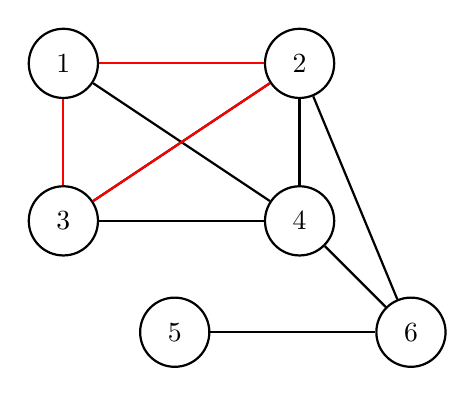
\begin{tikzpicture}[
    thick,
    node distance={35mm},
    auto
]

% nodes
\node[state] (1) {1};
\node[state] (2) [node distance=3cm, right of= 1]  {2};
\node[state] (3) [node distance=2cm, below of= 1] {3};
\node[state] (4) [node distance=2cm, below of= 2] {4};
\node[state] (5) [node distance=2cm, below right of= 3] {5};
\node[state] (6) [node distance=2cm, below right of= 4] {6};

% path
\path
    (1) edge[thick, red] (2)
    (1) edge[thick, red] (3)
    (1) edge (4)
    (2) edge (3)
    (2) edge (4)
    (3) edge (4)
    (3) edge[thick, red] (2)
    (5) edge (6)
    (6) edge (4)
    (6) edge (2)
    ;   

\end{tikzpicture} 
\end{document}

